\documentclass[11pt,a4paper]{article}
\usepackage[T1]{fontenc}
\usepackage[utf8]{inputenc}
\usepackage[brazil]{babel}
\usepackage{lmodern,microtype,graphicx,booktabs,longtable,array,xcolor}
\usepackage[margin=2.4cm]{geometry}
\usepackage[hidelinks]{hyperref}
\usepackage{float}
\renewcommand{\figurename}{Figura}
\renewcommand{\tablename}{Tabela}
\setlength{\parindent}{1cm}
\setlength{\parskip}{4pt}
\renewcommand{\arraystretch}{1.22}
\title{\textbf{Por Trás do Feed}\\\large Memorial do Projeto Final de Fundamentos de Informática}
\author{Davi Silva Vilaça\\CEFET-MG -- Campus Divinópolis\\Curso Técnico Integrado em Informática\\Professor: Alberto Pena Lara}
\date{10 de novembro de 2026}
\begin{document}
\maketitle
\begin{center}\textbf{Site publicado:}\\\url{https://vilaca-davi.github.io/por-tras-do-feed-fui/}\\[3pt]\textbf{Código do projeto:}\\\url{https://github.com/vilaca-davi/por-tras-do-feed-fui}\end{center}
\begin{abstract}
Criei o \textit{Por Trás do Feed}, um site educativo para mostrar como as curtidas podem mudar as recomendações de uma rede social fictícia. O visitante escolhe publicações, atualiza o feed e compara a quantidade de conteúdos de cada assunto. Neste memorial, explico a ideia, como o site foi desenvolvido, os testes realizados e a relação com os conteúdos de Fundamentos de Informática.
\end{abstract}
\section{Como surgiu a ideia}
A ideia do \textit{Por Trás do Feed} partiu de uma curiosidade sobre as redes sociais. Quando curtimos ou interagimos com um assunto, é comum perceber que outros conteúdos parecidos começam a aparecer. Isso me levou a pensar em como nossas escolhas podem influenciar aquilo que vemos na tela.

Decidi transformar essa pergunta em um site interativo. Em vez de mostrar apenas um texto sobre algoritmos, queria que a pessoa pudesse fazer uma experiência e observar a mudança acontecendo. O tema se relaciona com o cotidiano de quem utiliza redes sociais, inclusive estudantes. Esta é uma proposta de explicação da motivação do projeto, que representa o interesse que orientou a escolha do tema.

\section{O que eu quis criar}
Meu objetivo foi \textbf{criar um site que permitisse observar como curtidas mudam a distribuição de publicações em um feed simulado}. O site não tenta copiar o algoritmo de uma rede social real. Ele usa regras mais simples, justamente para que o visitante consiga entender o resultado.

O projeto foi feito como um site em HTML, CSS e JavaScript. Escolhi quatro categorias: tecnologia, música, esportes e cinema. No começo, aparecem duas publicações de cada categoria, totalizando oito vagas. Ao curtir uma publicação, a categoria ganha dois pontos. Depois de clicar em \textit{Atualizar feed}, o site recalcula quantas publicações de cada categoria aparecem.

Também incluí uma opção para reservar espaço para todas as categorias. Ela permite comparar um feed concentrado nos assuntos mais curtidos com outro que mantém alguma variedade.

\section{Como desenvolvi o site}
Primeiro organizei a proposta e as partes que o site precisava ter: uma apresentação do tema, uma animação explicativa e um laboratório interativo. Depois, trabalhei no visual, nas categorias e nas regras do simulador. Usei JavaScript para registrar as curtidas, calcular as pontuações e atualizar as quantidades exibidas.

Para deixar a explicação mais clara, usei cores diferentes para cada categoria e um painel que compara a distribuição inicial com a atual. O site também oferece exportação de dados em CSV. Organizei o planejamento em mapa mental, Trello e Obsidian, e publiquei o resultado no GitHub Pages.

\begin{figure}[H]\centering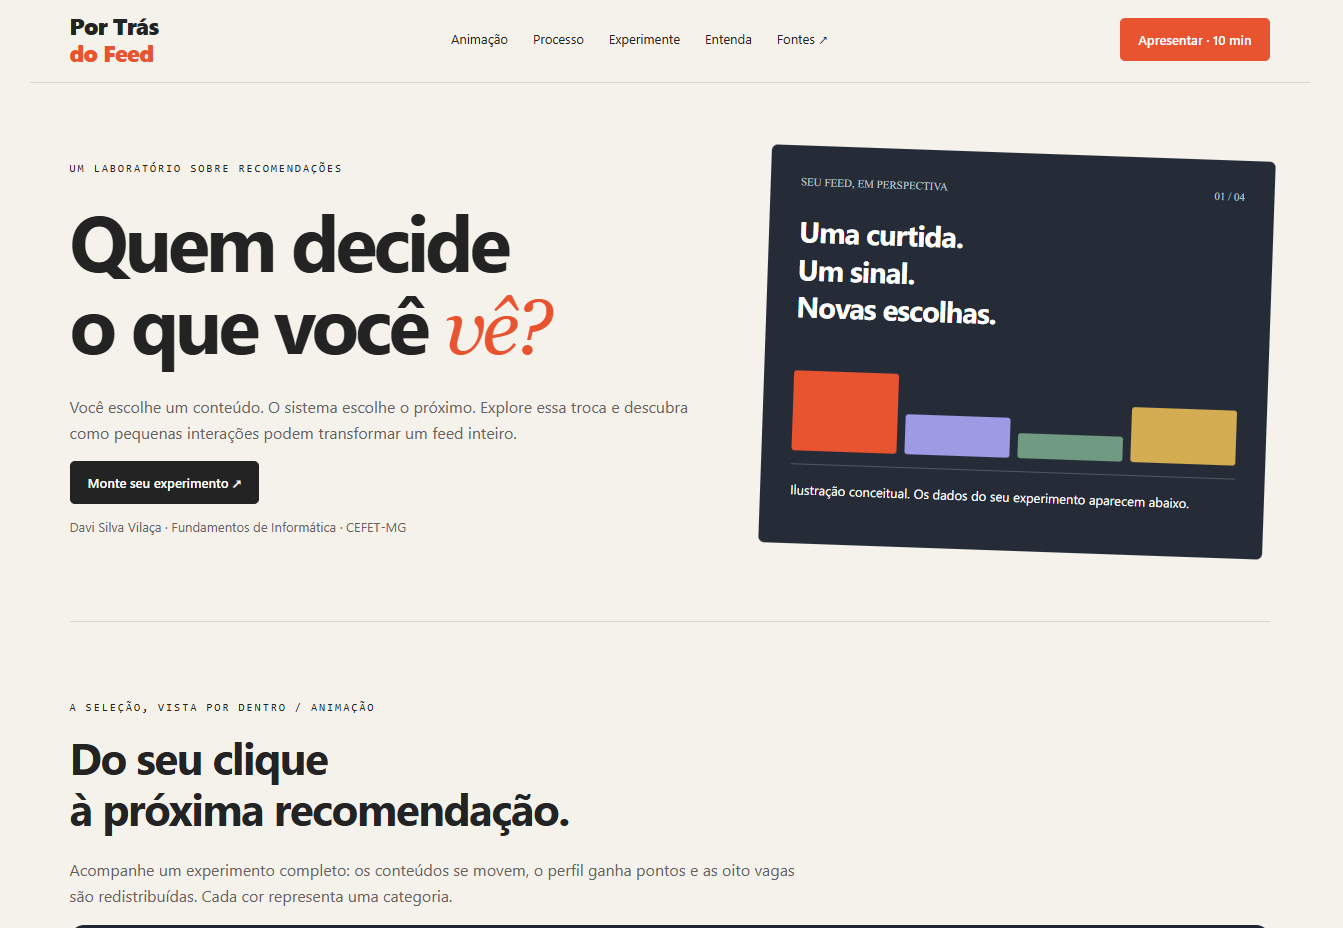
\includegraphics[width=0.96\linewidth]{inicio.png}\caption{Página inicial do site \textit{Por Trás do Feed}. Fonte: captura do projeto (2026).}\label{fig:inicio}\end{figure}

\begin{figure}[H]\centering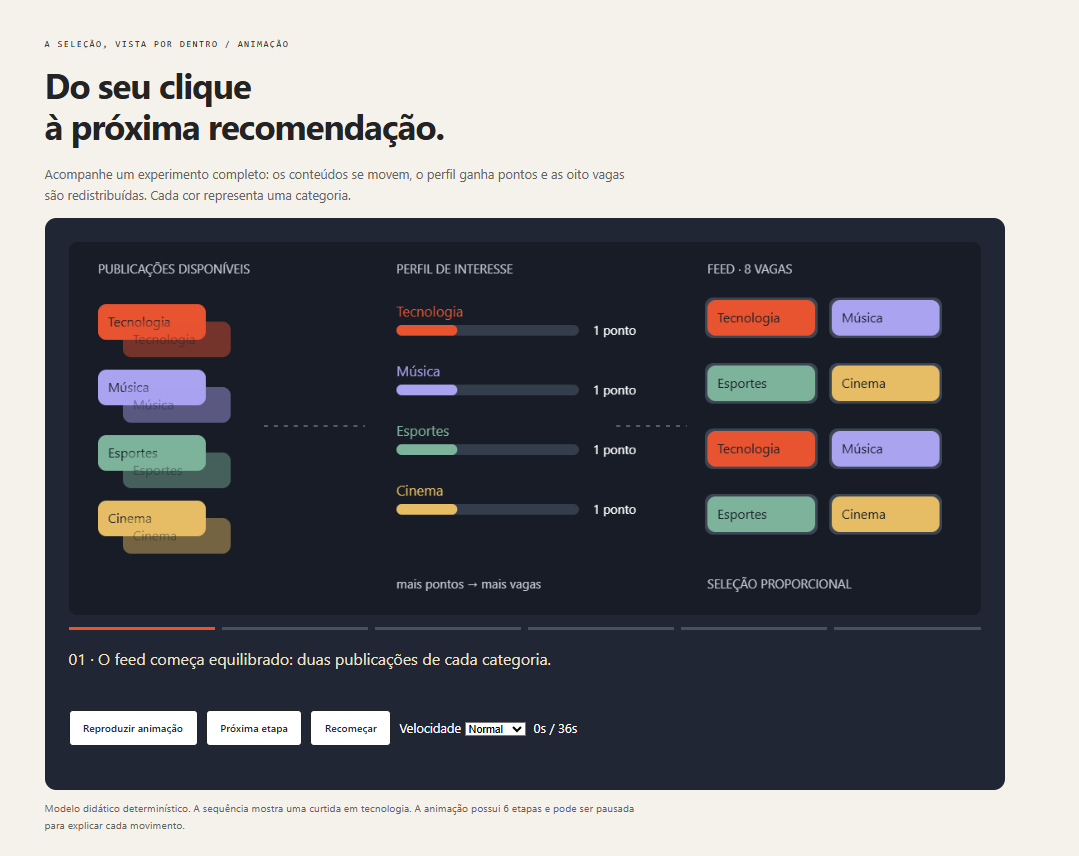
\includegraphics[width=0.88\linewidth]{animacao.png}\caption{Animação que explica, de forma visual, a relação entre interações e recomendações. Fonte: captura do projeto (2026).}\label{fig:animacao}\end{figure}

\section{O que aprendi e usei de FUI}
A Tabela~\ref{tab:matriz} mostra como relacionei os conteúdos da disciplina ao projeto. Procurei usar exemplos do próprio site e registrar evidências que podem ser conferidas.

\small
\begin{longtable}{>{\raggedright\arraybackslash}p{1.0cm}>{\raggedright\arraybackslash}p{4.0cm}>{\raggedright\arraybackslash}p{4.0cm}>{\raggedright\arraybackslash}p{5.1cm}}
\caption{Matriz de articulação dos conteúdos de FUI.}\label{tab:matriz}\\
\toprule Bloco & Atividade & Evidência & Contribuição \\\midrule\endfirsthead
\toprule Bloco & Atividade & Evidência & Contribuição \\\midrule\endhead
1A & Relacionei computadores e internet ao funcionamento de sites atuais. & Site publicado, Figura~\ref{fig:inicio}. & Situou o projeto como uma aplicação da informática no cotidiano. \\
1B & Trabalhei com valores e operações para distribuir oito vagas entre categorias. & Contagens e pontos, Figuras~\ref{fig:inicial} e~\ref{fig:resultado}. & Ajudou a representar e calcular os dados. A conversão explícita entre bases não foi documentada. \\
1C & Desenvolvi e testei o projeto em um computador pessoal. & Ambiente de desenvolvimento e arquivos do projeto. & Permitiu programar, testar e publicar o site. \\
1D & Usei cores digitais diferentes para as quatro categorias. & Figuras~\ref{fig:animacao} e~\ref{fig:inicial}. & Facilitou reconhecer os assuntos e comparar os resultados. \\
2B & Escrevi este memorial em LaTeX. & Arquivo \texttt{main.tex} e PDF. & Organizou texto, figuras e tabela. \\
2C & Usei referências cruzadas e registrei fontes. & Figuras e Tabela~\ref{tab:matriz} citadas no texto. & Tornou as evidências mais fáceis de localizar. \\
2D & Descrevi o problema e organizei as capturas. & Seções 2 e 4; Figuras~\ref{fig:inicio}--\ref{fig:resultado}. & Documentou o que o site procura explicar. \\
3B & Separei publicações por categoria e usei condições na simulação. & Simulador, Figura~\ref{fig:resultado}; código JavaScript. & Permitiu decidir como redistribuir as vagas. \\
3C & Incluí a exportação de arquivos CSV. & Botões de exportação na Figura~\ref{fig:inicial}. & Permitiu guardar e comparar dados do experimento. \\
3D & Criei representações visuais e uma animação, mas não um infográfico separado. & Figuras~\ref{fig:animacao} e~\ref{fig:resultado}. & Ajudou a explicar os dados visualmente. \\
3E & Organizei etapas em mapa mental, Trello e Obsidian. & Registros dessas ferramentas e notas do projeto. & Ajudou a acompanhar o desenvolvimento. \\
\bottomrule
\end{longtable}
\normalsize

\section{Testes e resultados}
Na Figura~\ref{fig:inicial}, o simulador começa com duas publicações de cada categoria e um ponto para cada assunto. A Figura~\ref{fig:resultado} registra um teste real depois de cinco curtidas e duas atualizações. Nesse teste, tecnologia passou de duas para cinco vagas, música ficou com uma, esportes com duas e cinema com zero.

\begin{figure}[H]\centering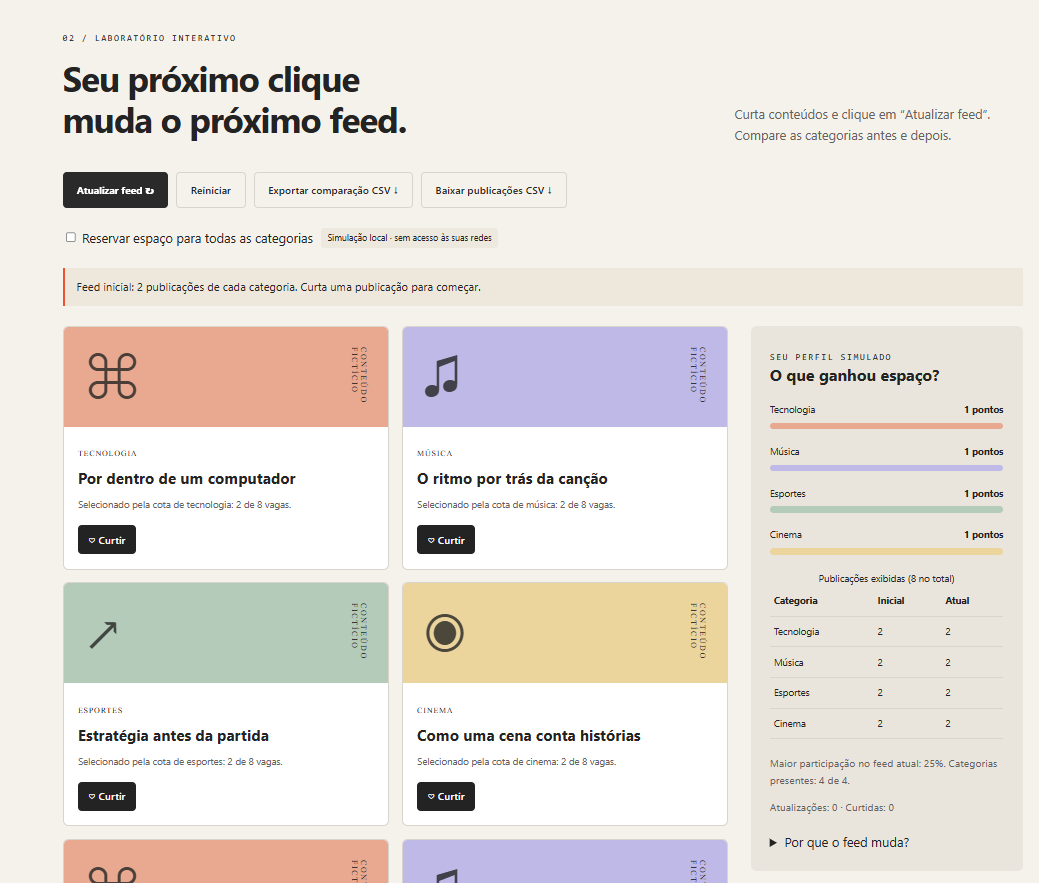
\includegraphics[width=0.87\linewidth]{feed_inicial.png}\caption{Simulador antes das interações, com duas vagas por categoria. Fonte: captura do projeto (2026).}\label{fig:inicial}\end{figure}
\begin{figure}[H]\centering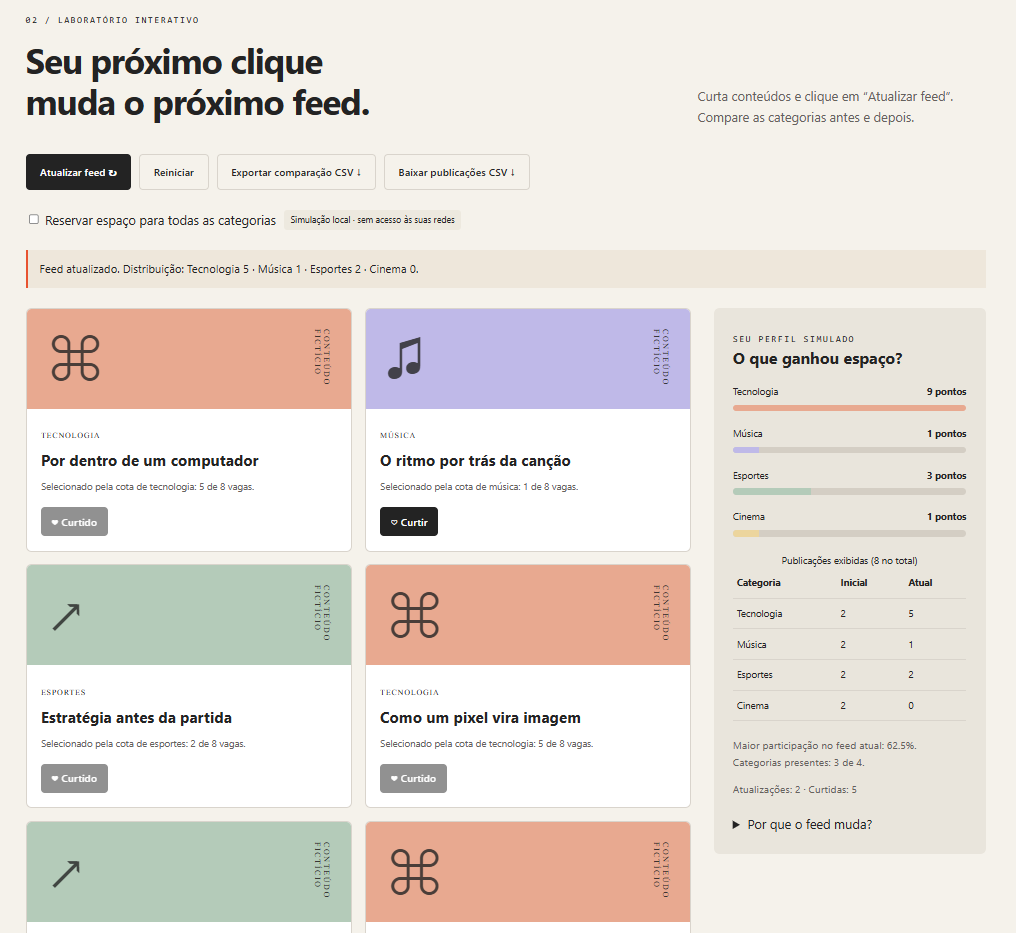
\includegraphics[width=0.87\linewidth]{feed_atualizado.png}\caption{Simulador após cinco curtidas e duas atualizações do feed. Fonte: captura do projeto (2026).}\label{fig:resultado}\end{figure}

\begin{table}[H]\centering\caption{Distribuição observada no teste.}\label{tab:resultado}\begin{tabular}{lrr}\toprule Categoria & Inicial & Após interações \\\midrule Tecnologia & 2 & 5 \\ Música & 2 & 1 \\ Esportes & 2 & 2 \\ Cinema & 2 & 0 \\\midrule Total & 8 & 8 \\\bottomrule\end{tabular}\end{table}

Esse resultado mostra como uma sequência de escolhas pode concentrar as recomendações em um assunto. No teste, tecnologia ocupou 62,5\% das oito vagas. Isso é uma demonstração didática, e não uma previsão do funcionamento das plataformas reais. Também testei a exportação CSV, que funcionou.

\section{Ferramentas, organização e uso de IA}
Usei HTML, CSS e JavaScript para o site; GitHub e GitHub Pages para guardar e publicar o projeto; mapa mental, Trello e Obsidian para planejar e registrar as etapas; e LaTeX para preparar este memorial. Usei inteligência artificial como apoio na organização das ideias, na escrita e revisão de textos e no desenvolvimento e ajuste do código. Conferi o funcionamento do simulador por meio de testes e capturas de tela. O projeto publicado e seus resultados são apresentados como um trabalho desenvolvido e verificado por mim com esse apoio.

\section{Conclusão}
O principal resultado foi conseguir transformar uma pergunta do cotidiano em um experimento que outras pessoas podem usar. Gostei especialmente de ver que uma ação simples, como curtir uma publicação, consegue alterar a distribuição do feed. O projeto também me ajudou a praticar programação, representação de dados, organização de arquivos e documentação. Se eu continuasse o desenvolvimento, poderia ampliar as categorias e criar novas formas de comparar os resultados.

\begin{thebibliography}{9}
\bibitem{enunciado} LARA, Alberto Pena. \textit{Trabalho final de Fundamentos de Informática}. CEFET-MG, 2026. Enunciado da disciplina.
\bibitem{github} GITHUB. \textit{GitHub Pages}. Disponível em: \url{https://docs.github.com/pt/pages}. Acesso em: 10 nov. 2026.
\bibitem{tiktok} TIKTOK. \textit{Como o TikTok recomenda conteúdo}. Disponível em: \url{https://support.tiktok.com/pt_BR/using-tiktok/exploring-videos/how-tiktok-recommends-content}. Material indicado para consulta sobre sistemas de recomendação.
\end{thebibliography}
\end{document}
